% $Header: /home/vedranm/bitbucket/beamer/solutions/conference-talks/conference-ornate-20min.en.tex,v 90e850259b8b 2007/01/28 20:48:30 tantau $

\documentclass[xcolor=dvipsnames]{beamer} 


% This file is a solution template for:

% - Talk at a conference/colloquium.
% - Talk length is about 20min.
% - Style is ornate.


% Copyright 2004 by Till Tantau <tantau@users.sourceforge.net>.
%
% In principle, this file can be redistributed and/or modified under
% the terms of the GNU Public License, version 2.
%
% However, this file is supposed to be a template to be modified
% for your own needs. For this reason, if you use this file as a
% template and not specifically distribute it as part of a another
% package/program, I grant the extra permission to freely copy and
% modify this file as you see fit and even to delete this copyright
% notice. 


\mode<presentation>
{
  %\usetheme{boxes}
  %\usecolortheme{seagull}
  % or ...

  \setbeamercovered{transparent}
  % or whatever (possibly just delete it)

    \usecolortheme[named=OliveGreen]{structure} 
    \usetheme[height=7mm]{Rochester} 
    \setbeamertemplate{items}[ball] 
    \setbeamertemplate{blocks}[rounded][shadow=true]
}


\usepackage[czech]{babel}
% or whatever
\usepackage{listings}

\usepackage[utf8]{inputenc}
% or whatever

\usepackage{hyperref}
%\definecolor{links}{HTML}{2A1B81}
\hypersetup{colorlinks,linkcolor=OliveGreen,urlcolor=OliveGreen}

\usepackage{times}
\usepackage[T1]{fontenc}
% Or whatever. Note that the encoding and the font should match. If T1
% does not look nice, try deleting the line with the fontenc.


\title[PyWPS-4] % (optional, use only with long paper titles)
{PyWPS 4}

\subtitle {Development restart}

\author[J. Čepický] % (optional, use only with lots of authors)
{Jáchym~Čepický\inst{1}}
% - Give the names in the same order as the appear in the paper.
% - Use the \inst{?} command only if the authors have different
%   affiliation.

\institute % (optional, but mostly needed)
{
  \inst{1}%
  \url{http://les-ejk.cz}\\
}
  
% - Use the \inst command only if there are several affiliations.
% - Keep it simple, no one is interested in your street address.

\date[] % (optional, should be abbreviation of conference name)
{Geoinformatics, Prague 2013}
% - Either use conference name or its abbreviation.
% - Not really informative to the audience, more for people (including
%   yourself) who are reading the slides online

% If you have a file called "university-logo-filename.xxx", where xxx
% is a graphic format that can be processed by latex or pdflatex,
% resp., then you can add a logo as follows:

\pgfdeclareimage[height=1.cm]{conference-logo}{images/conference-logo.png}
\pgfdeclareimage[height=1cm]{pywps-logo}{images/pywps.png}
%\pgfdeclareimage[height=2.0cm]{-logo}{university-logo-filename}
\logo{\pgfuseimage{conference-logo}}


% Delete this, if you do not want the table of contents to pop up at
% the beginning of each subsection:
\AtBeginSubsection[]
{
\logo{\pgfuseimage{conference-logo}}
  \begin{frame}<beamer>{Content}
    \tableofcontents[currentsection,currentsubsection]
  \end{frame}
}


% If you wish to uncover everything in a step-wise fashion, uncomment
% the following command: 

%\beamerdefaultoverlayspecification{<+->}


\begin{document}

\begin{frame}
  \titlepage
\end{frame}

\begin{frame}{TOC}
  \tableofcontents
  % You might wish to add the option [pausesections]
\end{frame}

\section{PyWPS}

\logo{\pgfuseimage{pywps-logo}}
\begin{frame}{PyWPS}
\begin{itemize} 
    \item OGC WPS on the Server
    \item Since 2006
    \item Python
    \item \url{http://pywps.wald.intevation.org}
    \item \url{http://github.org/geopython/pywps}
\end{itemize}
\end{frame}

\begin{frame}{PyWPS - what it is NOT}
    \alert{
        \begin{itemize}
            \item PyWPS is no analytical tool or engine. It does not perform any type of geospatial calculation.
                \pause
            \item PyWPS is not special XML parser or generator. It does not validate your GMLs against given schemas (yet), it does not build GML from Python objects.
                \pause
            \item It is not complicated
        \end{itemize}
    }
\end{frame}

\begin{frame}{Keywords}
    \begin{center}
        \only<2>{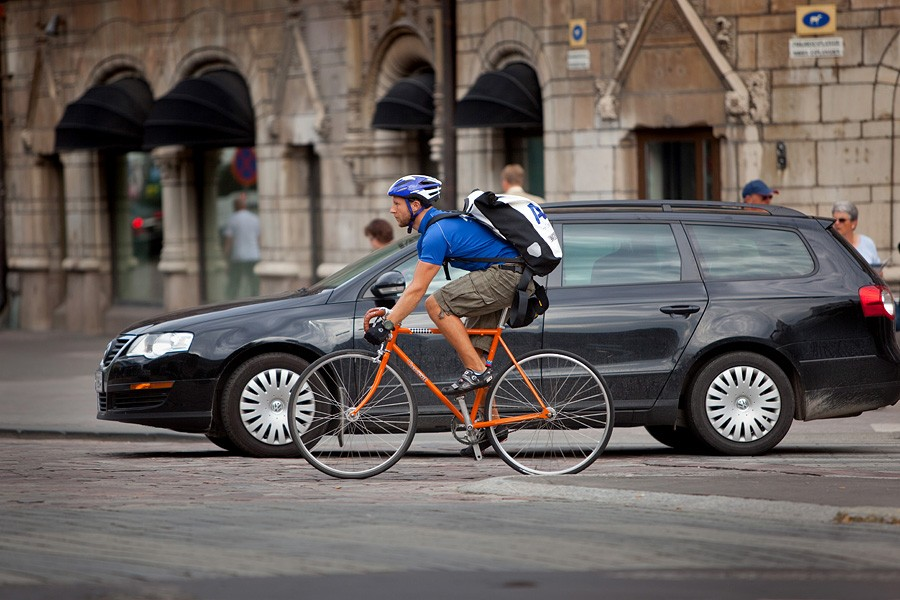
\includegraphics[width=\textwidth]{images/bike-car.jpg}\\
            rather bike, then a car}
        \only<3>{
\includegraphics[height=7cm]{images/small-bike.jpg}\\
            \#small}
        \only<4>{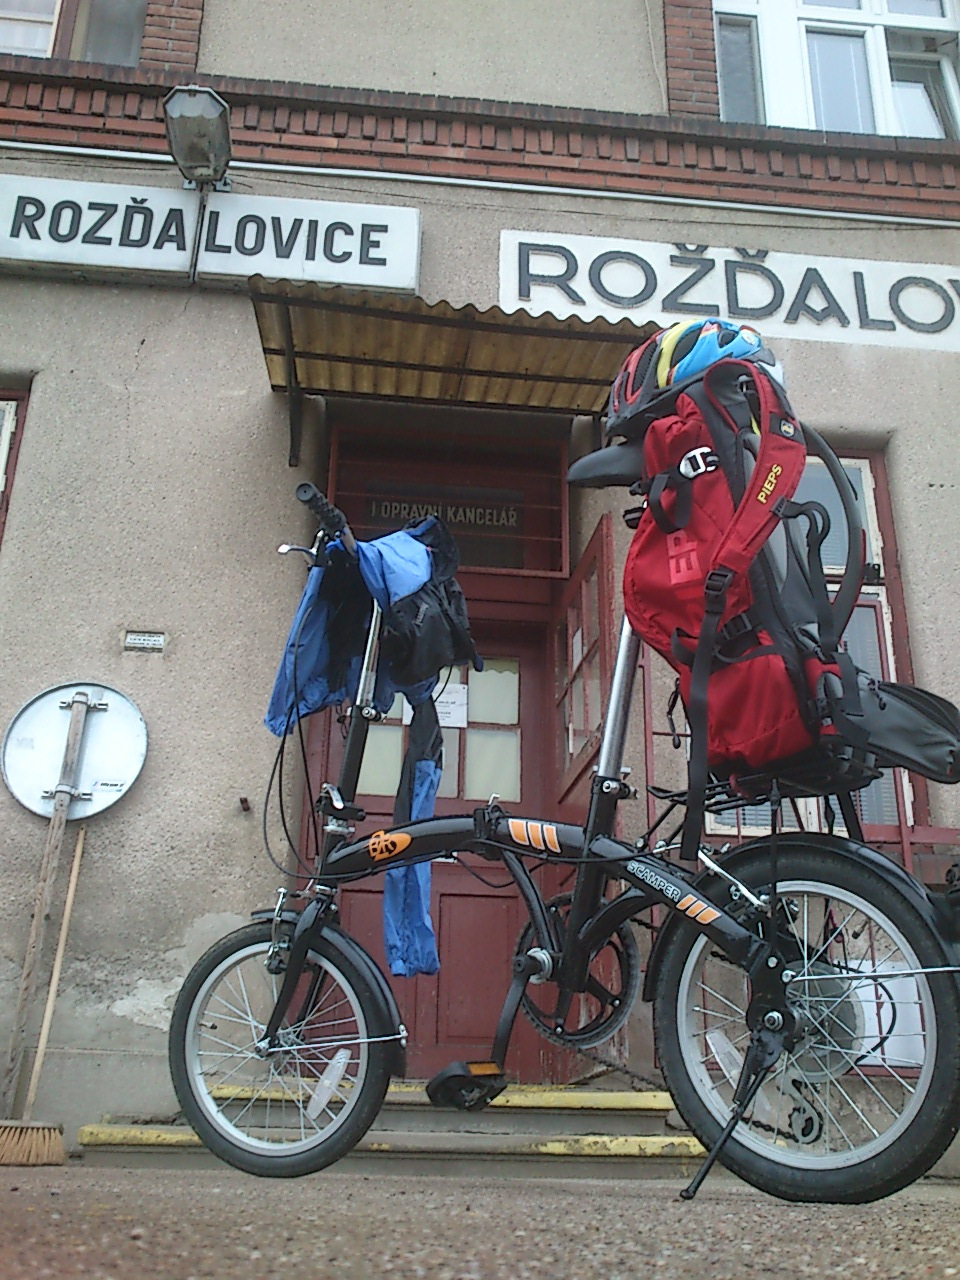
\includegraphics[height=7cm]{images/modular-bike.jpg}\\
            \#modular}
        \only<5>{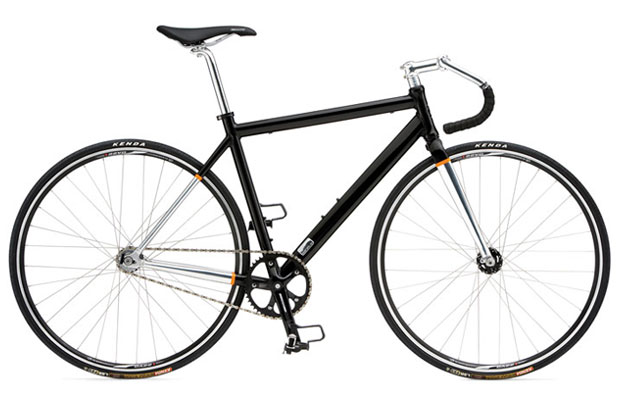
\includegraphics[width=\textwidth]{images/fast-bike.jpg}\\
            \#fast
        }
        \only<6>{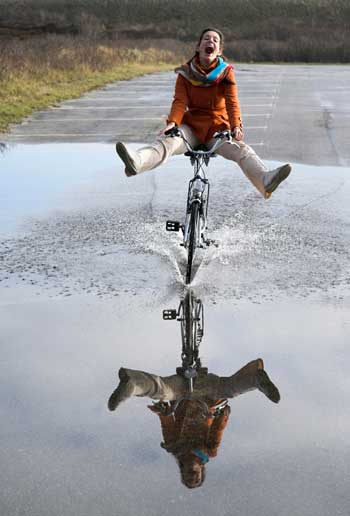
\includegraphics[height=7cm]{images/easy-bike.jpg}\\
            \#easy
        }
        \only<7>{
\includegraphics[height=7cm]{images/slick-bike.jpg}\\
            \#slick}
        \only<8>{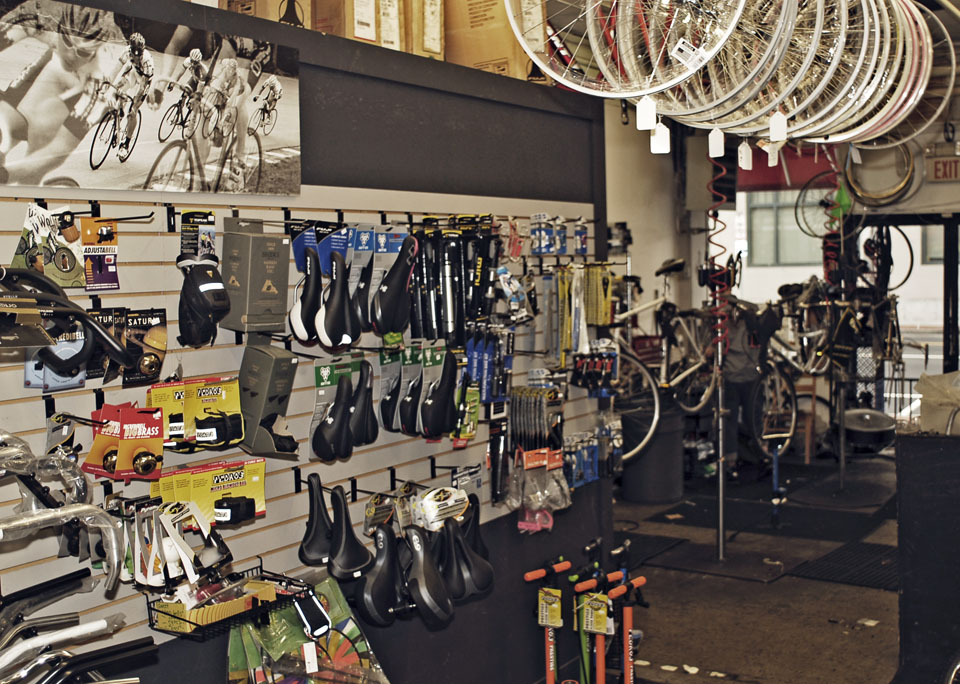
\includegraphics[height=7cm]{images/bike-accessories.jpg}\\
        \#accessories (GRASS, GDAL, Shapely, \#python)}
    \end{center}
\end{frame}

\section{PyWPS 4}
\begin{frame}{PyWPS 4}
    \begin{itemize}
        \item Started from scratch
            \pause
        \item Use Python 2.7 (for future 3.0 migration)
            \pause
        \item Try different interpreters of Python (pypy)
            \pause
        \item Easy parsing with lxml
            \pause
        \item Prepare for next WPS version
            \pause
        \item Change of the whole process concept
            \pause
    \end{itemize}
\end{frame}

\begin{frame}{PyWPS 4}
    \begin{center}
        \only<1>{
        
\includegraphics[height=7cm]{images/desert.jpg}\\
            \#geopython 2006
        }
        \only<2>{
        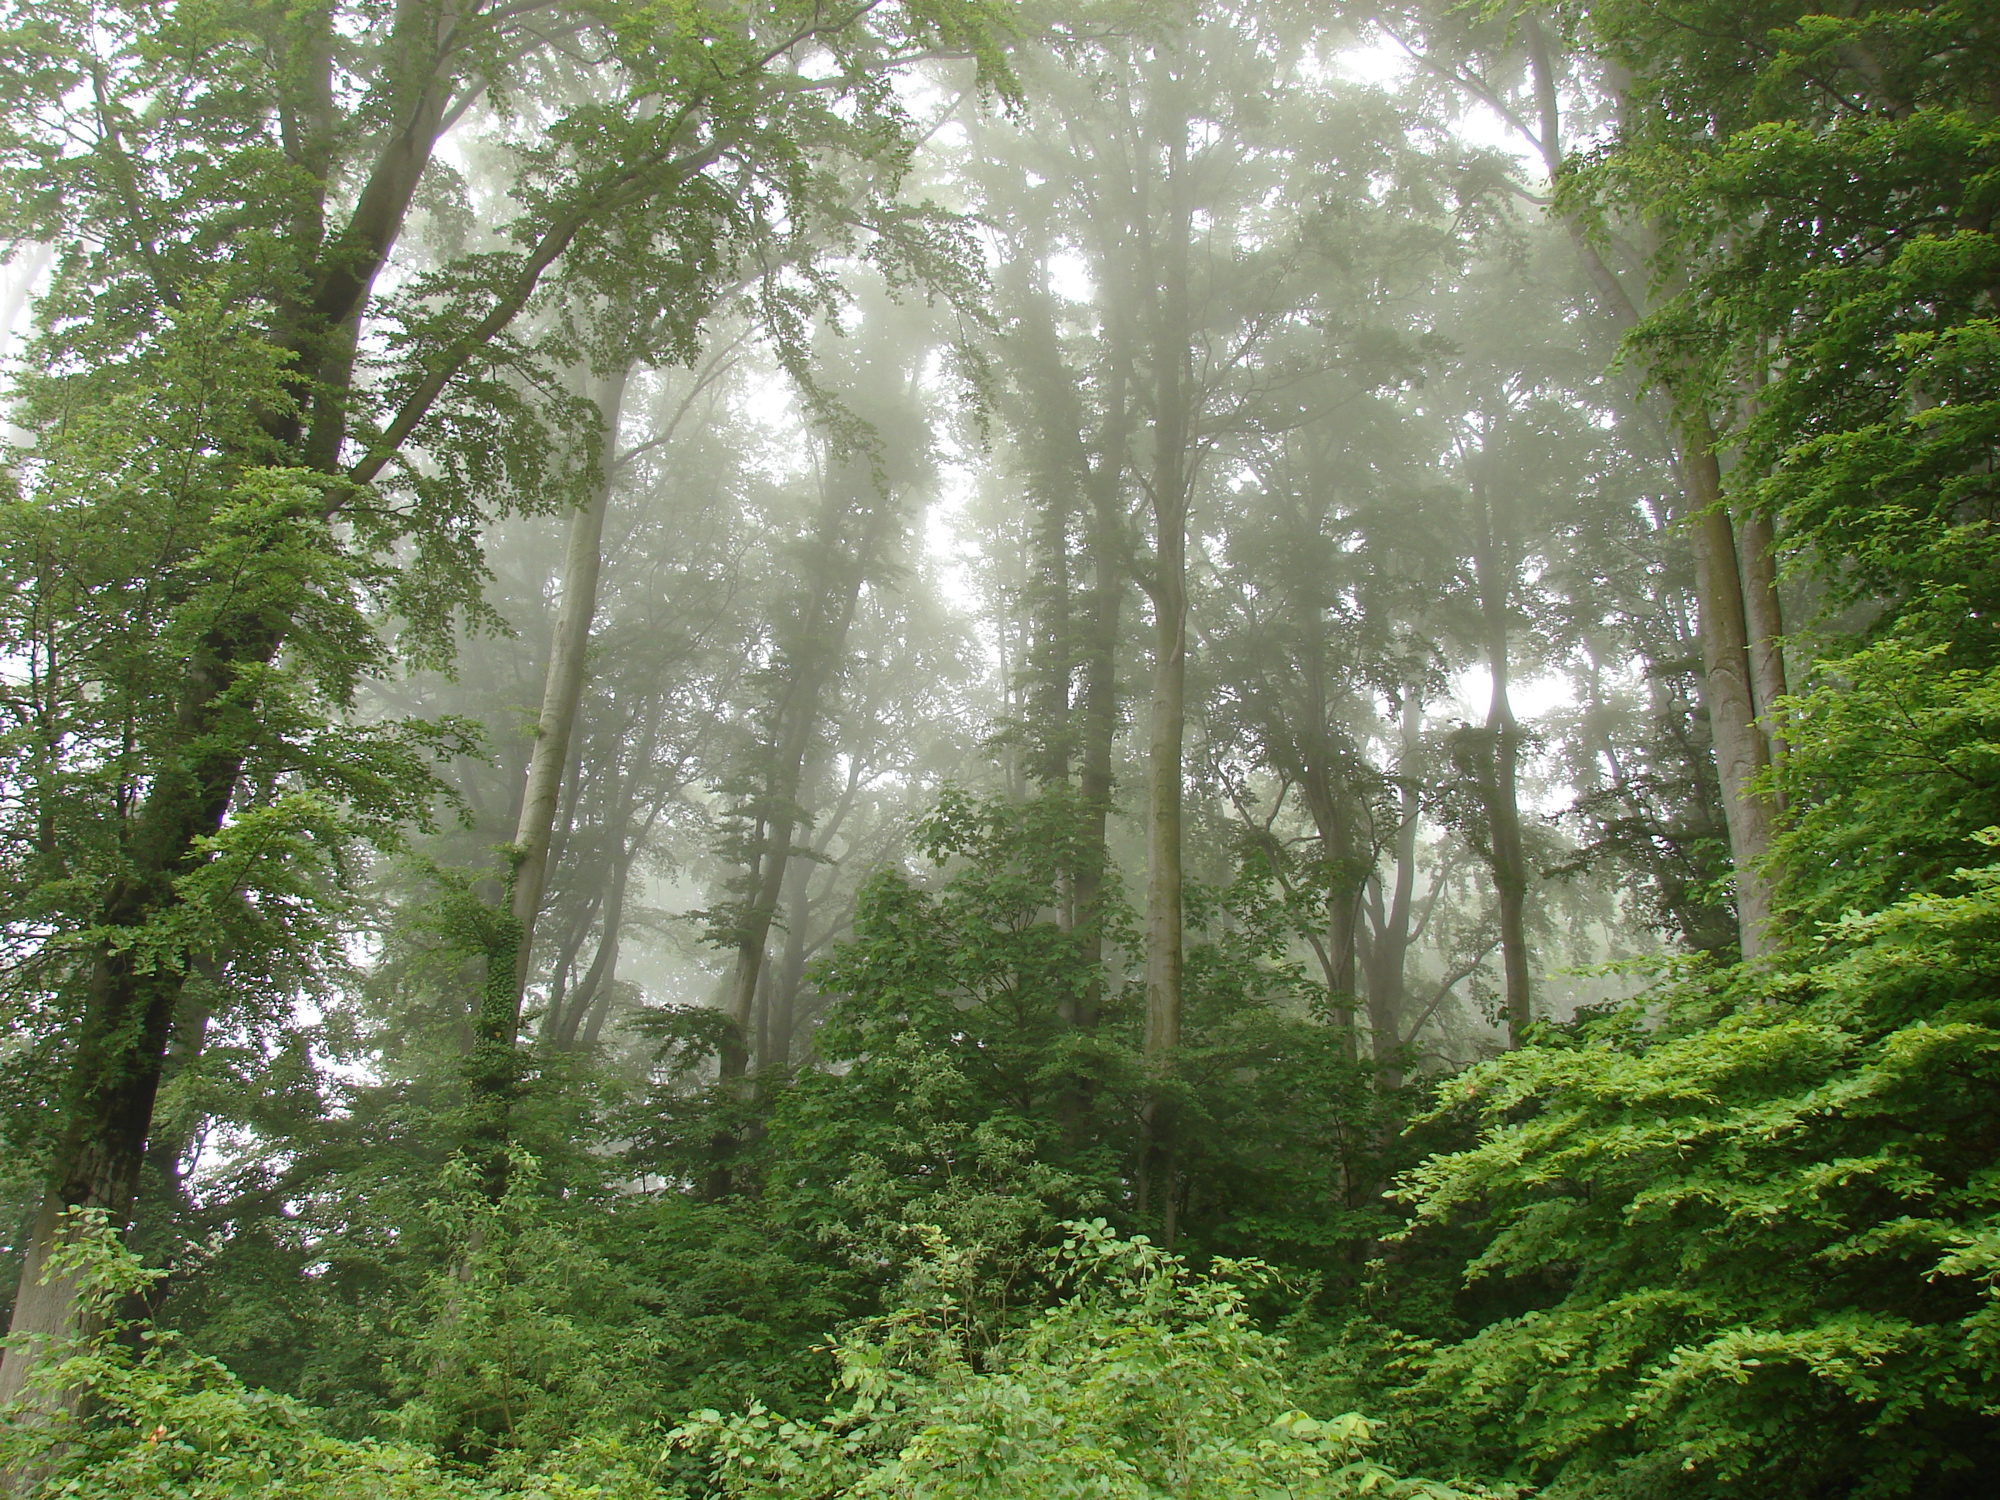
\includegraphics[height=7cm]{images/prales.jpg}\\
            \#geopython 2013
        }
    \end{center}
\end{frame}

\begin{frame}
    \begin{itemize}
        \item lxml \url{http://lxml.org}
        \item GRASS-WPS, GRASS-Python
        \item Werkzeug \url{http://werkzeug.pocoo.org/}
        \item Python 3
        \item Django
        \item \dots
    \end{itemize}
\end{frame}

\begin{frame}[fragile]{Process definition in PyWPS 3}
    \begin{lstlisting}[language=Python]
class Buffer(WPSProcess):
    def __init__(self):
        WPSProcess.__init__(self, identifier="buffer", ...)
        self.addComplexInput(identifier="input", ...)
        ...
        self.addLiteralOutpu(identifier="input", ...)
        ...
    def execute(self):
        ...
        return
    \end{lstlisting}
\end{frame}

\begin{frame}[fragile]{Process definition in PyWPS 4 (proposal)}
    \begin{itemize}
        \item 2-level APIs
        \item Providing the low-level API (integration with GRASS, writing a compatibility api for PyWPS-3, and defining a bunch of processes programatically if the user needs that. 
        \item The process is just a callable
        \item Inspired by Django
        \item Upper-level API for easy user-written processes
    \end{itemize}
\end{frame}

\begin{frame}[fragile]{PyWPS 4 - upper-level}
\begin{lstlisting}[language=Python]
class Buffer(pywps.Process):
     class Input:
        distance = pywps.Literal(value_type=pywps.Float)
        layer = pywps.Complex(as_file=True, max_occurs=None)
    class Output:
        feature_count = pywps.Literal(value_type=pywps.Integer)
        fortune = pywps.Literal(value_type
    def execute(self):
        ...
\end{lstlisting}
\end{frame}

\begin{frame}[fragile]{PyWPS 4 - low-level}
\begin{lstlisting}[language=Python]
def make_buffer(request):
    ...
make_buffer_process = pywps.create_process(
    identifier='makebuffer', title=...
    inputs=[
        pywps.Literal(identifier='distance', value_type=pywps.Float),
        pywps.BoundingBox(identifier='clip'),
    ],
    outputs=[
        pywps.Literal(identifier='feature_count', value_type=pywps.Integer),
        pywps.Literal(identifier='fortune', value_type=pywps.String),
    ],
    handler=make_buffer)
make_buffer_process()
\end{lstlisting}
\end{frame}

\begin{frame}{Where, what, how, who?}
    \begin{itemize}
        \item \url{http://github.org/jachym/pywps-4}
            \pause
        \item Tests, Basic request parsing, process definition, \dots
            \pause
        \item Alex Morega @mgax, Jorge de Jesus, Jachym Cepicky
            \pause
        \item \url{http://lists.osgeo.org/cgi-bin/mailman/listinfo/pywps-dev}
    \end{itemize}
\end{frame}

\section*{Closing}
\begin{frame}
    \begin{center}
        thank you!\\
        jachym@les-ejk.cz\\
        \url{http://github.org/jachym/pywps-4}\\
        \bigskip
        questions?
    \end{center}
\end{frame}
    

\end{document}
